\subsection{Diagrama de Casos de Uso}

\begin{figure}[H]
    \centering
    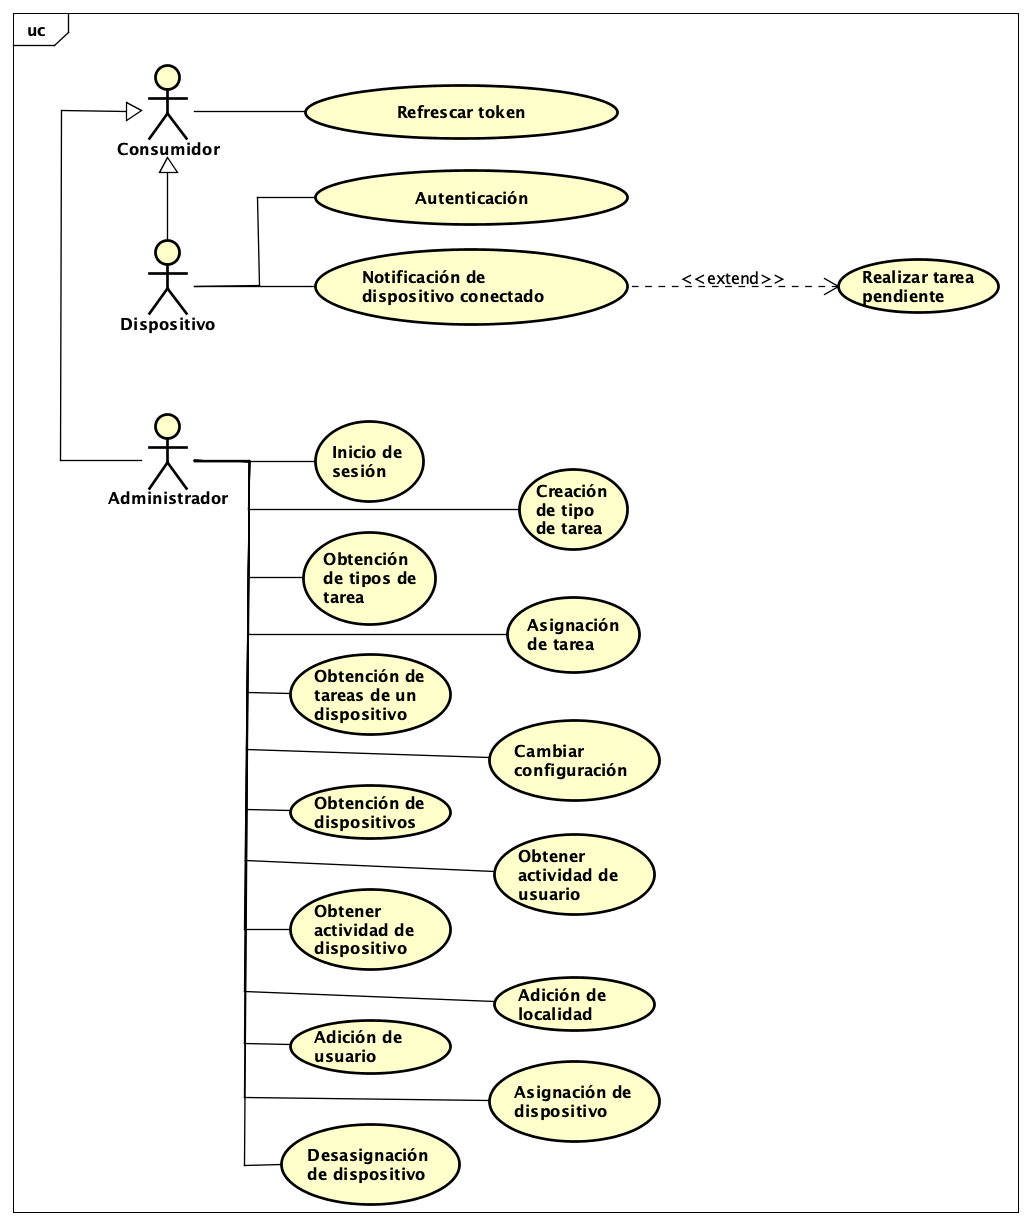
\includegraphics[width=14cm]{./img/uc.png}
    \caption{Diagrama general de casos de uso}
    \label{fig:seq.alive}
\end{figure}

\subsection{Definición de Casos de Uso}

%% ====== DISPOSITIVO ======

%% IDENTIFICAR DISPOSITIVO
\begin{table}[H]
\centering
	\setlength{\extrarowheight}{3pt}
		\begin{tabular}{rc{1.85cm}|Y{8cm}}
	    \hline
        \multicolumn{1}{|l}{ CU_D01 }     & \multicolumn{1}{Y|}{\textbf{Inicio de sesión}  } \\
	    \hline \hline
	    \multicolumn{1}{|l}{Descripción}     & \multicolumn{1}{Y|}{
	    Un dispositivo se identifica ante el sistema con el fin de obtener unos tokens de acceso, con los que autenticar posteriormente sus llamadas.
	    }  \\ \cline{1-2}
	    \multicolumn{1}{|l}{Actor}           & \multicolumn{1}{Y|}{Dispositivo}  \\ \cline{1-2}
	    \multicolumn{1}{|l}{Precondiciones}  & \multicolumn{1}{Y|}{El dispositivo tiene conexión a Internet.}  \\ \cline{1-2}
	    \multicolumn{1}{|l}{Postcondiciones} & \multicolumn{1}{Y|}{Se obtiene un par de tokens.}\\ \cline{1-2}
	    \multicolumn{1}{|l}{Flujo normal}    & \multicolumn{1}{Y|}{
1. El dispositivo obtiene su dirección MAC.\newline
2. El dispositivo genera la clave a partir de una encriptación de su MAC, formando sus credenciales, y se las envía al servidor. \newline
3. El servidor comprueba la validez de las credenciales, genera un par de tokens asociados al dispositivo y los devuelve. \newline
4. El dispositivo almacena los tokens y finaliza el caso de uso.
	    } \\ \cline{1-2}
	    \multicolumn{1}{|l}{Flujo Alternativo} & \multicolumn{1}{Y|}{
	    \textbf{Flujo alternativo 1:} \newline
3.A1.1. El servidor comprueba que los credenciales no son válidos y devuelve error. \newline
3.A1.2. El dispositivo recibe el error y finaliza el caso de uso. \newline\newline
	    \textbf{Flujo alternativo 2:} \newline
3.A2.1. El servidor detecta que las credenciales son válidas pero no hay ningún registro del dispositivo.\newline
3.A2.2. El servidor registra el nuevo dispositivo, genera un par de tokens asociados a su identificador y los devuelve.
}\\ \cline{1-2}
	    \hline
	    \end{tabular}
	\label{table:cu_d01}
	\caption{Caso de Uso D01 - Inicio de sesión}
\end{table}

%%%% REFRESH TOKEN
\begin{table}[H]
\centering
	\setlength{\extrarowheight}{3pt}
		\begin{tabular}{rc{1.85cm}|c{8cm}}
	    \hline
        \multicolumn{1}{|l}{CU_U01}     & \multicolumn{1}{Y|}{\textbf{Refresco de token de acceso}  } \\
	    \hline \hline
	    \multicolumn{1}{|l}{Descripción}     & \multicolumn{1}{Y|}{
	    Un dispositivo o usuario piden al servidor una actualización de sus tokens de acceso.
	    }  \\ \cline{1-2}
	    \multicolumn{1}{|l}{Actor}           & \multicolumn{1}{Y|}{Usuario}  \\ \cline{1-2}
	    \multicolumn{1}{|l}{Precondiciones}  & \multicolumn{1}{Y|}{
1. El usuario tiene conexión a Internet.\newline
2. El dispositivo tiene un token de refresco válido.}  \\ \cline{1-2}
	    \multicolumn{1}{|l}{Postcondiciones} & \multicolumn{1}{Y|}{Se obtiene un par de tokens.}\\ \cline{1-2}
	    \multicolumn{1}{|l}{Flujo normal}    & \multicolumn{1}{Y|}{
1. El usuario manda su token de refresco. \newline
2. El sistema comprueba la validez del token de refresco, obtiene la información sobre el usuario, le asocia un par nuevo de tokens y los devuelve. \newline
3. El usuario recibe los tokens nuevos de acceso y finaliza el caso de uso.
	    } \\ \cline{1-2}
	    \multicolumn{1}{|l}{Flujo Alternativo} & \multicolumn{1}{Y|}{
2.A1.1. El sistema comprueba que el token de refresco no es válido y responde un mensaje de error. \newline
2.A1.2. El usuario recibe el error, descarta los tokens que tenía almacenados y finaliza el caso de uso.
}\\ \cline{1-2}
	    \hline
	    \end{tabular}
	\label{table:cu_u01}
	\caption{Caso de Uso U01 - Refresco de token de acceso}
\end{table}


%%%% AVISO ACTIVO + TAREA

\begin{table}[H]
\centering
	\setlength{\extrarowheight}{3pt}
		\begin{tabular}{r{1.85cm}|Y}
	    \hline
        \multicolumn{1}{|l}{CU_D02}     & \multicolumn{1}{Y|}{\textbf{Notificación de dispositivo conectado} } \\
	    \hline \hline
	    \multicolumn{1}{|l}{Descripción}     & \multicolumn{1}{Y|}{
	    Un dispositivo avisa de que está encendido.
	    }  \\ \cline{1-2}
	    \multicolumn{1}{|l}{Actor}           & \multicolumn{1}{Y|}{Dispositivo}  \\ \cline{1-2}
	    \multicolumn{1}{|l}{Precondiciones}  & \multicolumn{1}{Y|}{
1. El dispositivo tiene conexión a Internet.\newline
2. El dispositivo tiene un par de tokens activos.}  \\ \cline{1-2}
	    \multicolumn{1}{|l}{Postcondiciones} & \multicolumn{1}{Y|}{
1. El sistema actualiza su registro.}\\ \cline{1-2}
	    \multicolumn{1}{|l}{Flujo normal}    & \multicolumn{1}{Y|}{
1. El dispositivo hace una petición \textit{/alive} al servidor. \newline
2. El sistema recibe la llamada, valida los credenciales, comprueba que no hay ninguna tarea pendiente, y responde al dispositivo. \newline
3. El dispositivo recibe una respuesta vacía del servidor. \newline
4. Finaliza el caso de uso.
	    } \\ \cline{1-2}
	    \multicolumn{1}{|l}{Flujo Alternativo} & \multicolumn{1}{Y|}{
2.A1.1. El sistema detecta que el dispositivo tiene tareas asignadas pendientes, de modo que las recolecta y devuelve.\newline
2.A1.2. Se realiza el caso de uso \textit{Realizar tarea pendiente}.\newline
2.A1.3. Finaliza el caso de uso.
	    }\\ \cline{1-2}
	    \hline
	    \end{tabular}
	\label{table:cu-d-02}
	\caption{Caso de Uso D02 - Notificación de dispositivo conectado.}
\end{table}

%% Realizar tarea 

\begin{table}[H]
\centering
	\setlength{\extrarowheight}{3pt}
		\begin{tabular}{r{1.85cm}|Y}
	    \hline
        \multicolumn{1}{|l}{CU_D03}     & \multicolumn{1}{Y|}{\textbf{Realización de tarea pendiente} } \\
	    \hline \hline
	    \multicolumn{1}{|l}{Descripción}     & \multicolumn{1}{Y|}{
	    El dispositivo ejecuta una acción pendiente.
	    }  \\ \cline{1-2}
	    \multicolumn{1}{|l}{Actor}           & \multicolumn{1}{Y|}{Dispositivo}  \\ \cline{1-2}
	    \multicolumn{1}{|l}{Precondiciones}  & \multicolumn{1}{Y|}{
1. El dispositivo tiene conexión a Internet.\newline
2. El dispositivo ha recibido una lista de tareas pendientes.}  \\ \cline{1-2}
	    \multicolumn{1}{|l}{Postcondiciones} & \multicolumn{1}{Y|}{
1. El sistema actualiza su registro.}\\ \cline{1-2}
	    \multicolumn{1}{|l}{Flujo normal}    & \multicolumn{1}{Y|}{
1. El dispositivo recibe una lista de tareas pendientes. \newline
2. El dispositivo avisa al servidor que va a hacer la tarea. \newline
3. El servidor marca la tarea como realizada y actualiza su registro del estado del dispositivo.\newline
3. El dispositivo hace la tarea. \newline
4. Finaliza el caso de uso.
	    } \\ \cline{1-2}
	    \multicolumn{1}{|l}{Flujo Alternativo} & \multicolumn{1}{Y|}{

	    }\\ \cline{1-2}
	    \hline
	    \end{tabular}
	\label{table:cu-d-03}
	\caption{Caso de Uso D03 - Realización de tarea pendiente.}
\end{table}

%% OBTENER CONFIGURACIÓN

\begin{table}[H]
\centering
	\setlength{\extrarowheight}{3pt}
		\begin{tabular}{r{1.85cm}|Y}
	    \hline
        \multicolumn{1}{|l}{CU_D04}     & \multicolumn{1}{Y|}{\textbf{Actualización de configuración} } \\
	    \hline \hline
	    \multicolumn{1}{|l}{Descripción}     & \multicolumn{1}{Y|}{
	    El dispositivo actualiza su configuración.
	    }  \\ \cline{1-2}
	    \multicolumn{1}{|l}{Actor}           & \multicolumn{1}{Y|}{Dispositivo}  \\ \cline{1-2}
	    \multicolumn{1}{|l}{Precondiciones}  & \multicolumn{1}{Y|}{
1. El dispositivo tiene conexión a Internet.\newline
2. El dispositivo tiene un token de acceso válido.}  \\ \cline{1-2}
	    \multicolumn{1}{|l}{Postcondiciones} & \multicolumn{1}{Y|}{
1. El dispositivo actualiza su fichero de configuración. \newline
2. El servidor actualiza el registro de configuraciones.}\\ \cline{1-2}
	    \multicolumn{1}{|l}{Flujo normal}    & \multicolumn{1}{Y|}{
1. El dispositivo solicita al servidor obtener la configuración. \newline
2. El servidor obtiene la configuración añadida recientemente que aún no haya recogido el dispositivo, obteniendo la identificación del dispositivo a partir de su token de acceso, y se la devuelve. \newline
3. El dispositivo obtiene su configuración, actualiza el fichero donde la guarda e informa al servidor acerca de la completitud. \newline
4. El servidor actualiza sus registros de actualizaciones e informa al dispositivo. \newline
5. El dispositivo recibe esa respuesta y finaliza el caso de uso. \newline
	    } \\ \cline{1-2}
	    \multicolumn{1}{|l}{Flujo Alternativo} & \multicolumn{1}{Y|}{
2.A1.1. El servidor detecta que el dispositivo tiene ya la configuración más reciente por lo que le devuelve un mensaje vacío. \newline
2.A1.2. El dispositivo recibe el mensaje vacío, y finaliza el caso de uso. \newline

	    }\\ \cline{1-2}
	    \hline
	    \end{tabular}
	\label{table:cu-d-04}
	\caption{Caso de Uso D04 - Actualización de configuración}
\end{table}

%% ADICION DE ACTIVIDAD DE DISPOSITIVO

\begin{table}[H]
\centering
	\setlength{\extrarowheight}{3pt}
		\begin{tabular}{r{1.85cm}|Y}
	    \hline
        \multicolumn{1}{|l}{CU_D05}     & \multicolumn{1}{Y|}{\textbf{Envío de actividad de un dispositivo} } \\
	    \hline \hline
	    \multicolumn{1}{|l}{Descripción}     & \multicolumn{1}{Y|}{
	    El dispositivo envía su actividad al servidor.
	    }  \\ \cline{1-2}
	    \multicolumn{1}{|l}{Actor}           & \multicolumn{1}{Y|}{Dispositivo}  \\ \cline{1-2}
	    \multicolumn{1}{|l}{Precondiciones}  & \multicolumn{1}{Y|}{
1. El dispositivo tiene conexión a Internet.\newline
2. El dispositivo tiene un token de acceso válido.\newline
3. El dispositivo ha realizado alguna actividad con el usuario.}\\ \cline{1-2}
	    \multicolumn{1}{|l}{Postcondiciones} & \multicolumn{1}{Y|}{
1. El servidor actualiza su registro de actividades.}\\ \cline{1-2}
	    \multicolumn{1}{|l}{Flujo normal}    & \multicolumn{1}{Y|}{
1. El dispositivo procesa una nueva actividad y la envía al servidor. \newline
2. El servidor autentica al dispositivo a partir de su token, comprueba la validez de los datos enviados, registra la actividad asignando una marca de tiempo a dicha actividad, y devuelve un mensaje de confirmación al dispositivo. \newline
3. El dispositivo recibe esa respuesta y finaliza el caso de uso. \newline
	    } \\ \cline{1-2}
	    \multicolumn{1}{|l}{Flujo Alternativo} & \multicolumn{1}{Y|}{
2.A1.1. El servidor detecta que la autenticación no es válida y devuelve error. \newline
2.A1.2. El dispositivo recibe un mensaje no válido, y devuelve error. \newline

	    }\\ \cline{1-2}
	    \hline
	    \end{tabular}
	\label{table:cu-d-05}
	\caption{Caso de Uso D05 - Envío de actividad de un dispositivo}
\end{table}

%% ADMINISTRADOR INICIO SESIÓN

\begin{table}[H]
\centering
	\setlength{\extrarowheight}{3pt}
		\begin{tabular}{rc{1.85cm}|Y{8cm}}
	    \hline
        \multicolumn{1}{|l}{CU_A01}     & \multicolumn{1}{Y|}{\textbf{Inicio de sesión}  } \\
	    \hline \hline
	    \multicolumn{1}{|l}{Descripción}     & \multicolumn{1}{Y|}{
	    Un administrador se identifica ante el sistema con el fin de obtener unos tokens de acceso, con los que autenticar posteriormente sus llamadas.
	    }  \\ \cline{1-2}
	    \multicolumn{1}{|l}{Actor}           & \multicolumn{1}{Y|}{Administrador}  \\ \cline{1-2}
	    \multicolumn{1}{|l}{Precondiciones}  & \multicolumn{1}{Y|}{El administrador tiene conexión a Internet.}  \\ \cline{1-2}
	    \multicolumn{1}{|l}{Postcondiciones} & \multicolumn{1}{Y|}{El administrador obtiene un par de tokens.}\\ \cline{1-2}
	    \multicolumn{1}{|l}{Flujo normal}    & \multicolumn{1}{Y|}{
1. El administrador envía sus credenciales al servidor.\newline
2. El servidor comprueba la validez de las credenciales, genera un par de tokens asociados al administrador, y los devuelve. \newline
3. El administrador almacena los tokens y finaliza el caso de uso.
	    } \\ \cline{1-2}
	    \multicolumn{1}{|l}{Flujo Alternativo} & \multicolumn{1}{Y|}{
2.A1.1. El servidor comprueba que los credenciales no son válidos y devuelve error. \newline
2.A1.2. El administrador recibe el error y finaliza el caso de uso.\newline
}\\ \cline{1-2}
	    \hline
	    \end{tabular}
	\label{table:cu_A01}
	\caption{Caso de Uso A01 - Inicio de sesión}
\end{table}


%% CREAR NUEVO TIPO DE TAREA
    %% BACK
\begin{table}[H]
\centering
	\setlength{\extrarowheight}{3pt}
		\begin{tabular}{rc{1.85cm}|Y{8cm}}
	    \hline
        \multicolumn{1}{|l}{CU_A02}     & \multicolumn{1}{Y|}{\textbf{Creacción de un nuevo tipo de tarea}  } \\
	    \hline \hline
	    \multicolumn{1}{|l}{Descripción}     & \multicolumn{1}{Y|}{
	    Un administrador crea un nuevo tipo de tarea que será asignable a un dispositivo.
	    }  \\ \cline{1-2}
	    \multicolumn{1}{|l}{Actor}           & \multicolumn{1}{Y|}{Administrador}  \\ \cline{1-2}
	    \multicolumn{1}{|l}{Precondiciones}  & \multicolumn{1}{Y|}{
El administrador posee un token de acceso activo.}  \\ \cline{1-2}
	    \multicolumn{1}{|l}{Postcondiciones} & \multicolumn{1}{Y|}{
Se registra un nuevo tipo de tarea.}\\ \cline{1-2}
	    \multicolumn{1}{|l}{Flujo normal}    & \multicolumn{1}{Y|}{
1. El administrador envía un nuevo tipo de tarea y el contenido de esta al servidor.\newline
2. El servidor autentica la petición, comprueba el contenido recibido, crea un nuevo tipo de tarea, e informa sobre la completitud. \newline
3. El administrador recibe el mensaje y finaliza el caso de uso. \newline
	    } \\ \cline{1-2}
	    \multicolumn{1}{|l}{Flujo Alternativo} & \multicolumn{1}{Y|}{
	    \textbf{Flujo Alternativo 1:} \newline
2.A1.1. El servidor comprueba que los credenciales no son válidos y devuelve error. \newline

	    \textbf{Flujo Alternativo 2:} \newline
2.A2.1. El servidor detecta un error en la información introducida y devuelve error. \newline }
\\ \cline{1-2}
	    \hline
	    \end{tabular}
	\label{table:cu_A02}
	\caption{Caso de Uso A02 - Creacción de un nuevo tipo de tarea.}
\end{table}
    %% FRONT
    
    

%%%% Asignación de tarea

\begin{table}[H]
\centering
	\setlength{\extrarowheight}{3pt}
		\begin{tabular}{r{1.85cm}|Y}
	    \hline
        \multicolumn{1}{|l}{CU_A03}     & \multicolumn{1}{Y|}{\textbf{Asignación de tarea} } \\
	    \hline \hline
	    \multicolumn{1}{|l}{Descripción}     & \multicolumn{1}{Y|}{
	    Un administrador asigna una nueva tarea a un dispositivo específico.
	    }  \\ \cline{1-2}
	    \multicolumn{1}{|l}{Actor}           & \multicolumn{1}{Y|}{Dispositivo}  \\ \cline{1-2}
	    \multicolumn{1}{|l}{Precondiciones}  & \multicolumn{1}{Y|}{
1. El administrador está autenticado ante el sistema.}\\ \cline{1-2}
	    \multicolumn{1}{|l}{Postcondiciones} & \multicolumn{1}{Y|}{
1. Se registra una nueva tarea como pendiente para un dispositivo específico.
}\\ \cline{1-2}
	    \multicolumn{1}{|l}{Flujo normal}    & \multicolumn{1}{Y|}{
1. El administrador selecciona un dispositivo específico, selecciona una tarea, y la envía. \newline
2. El sistema recibe una nueva asignación de tarea, comprueba que es una petición autenticada, asigna la tarea como pendiente para el dispositivo y responde como petición correcta. \newline
3. El administrador recibe la respuesta y finaliza el caso de uso. \newline} \\ \cline{1-2}
	    \multicolumn{1}{|l}{Flujo Alternativo} & \multicolumn{1}{Y|}{
        }\\ \cline{1-2}
	    \hline
	    \end{tabular}
	\label{table:cu-a-03}
	\caption{Caso de Uso A03 - Asignación de nueva tarea.}
\end{table}
    
%% VER TAREAS EXISTENTES
\begin{table}[H]
\centering
	\setlength{\extrarowheight}{3pt}
		\begin{tabular}{rc{1.85cm}|Y{8cm}}
	    \hline
        \multicolumn{1}{|l}{CU_A04}     & \multicolumn{1}{Y|}{\textbf{Recolectar tareas existentes}  } \\
	    \hline \hline
	    \multicolumn{1}{|l}{Descripción}     & \multicolumn{1}{Y|}{
	    Un administrador obtiene una lista con todas las tareas existentes asignables a dispositivos.
	    }  \\ \cline{1-2}
	    \multicolumn{1}{|l}{Actor}           & \multicolumn{1}{Y|}{Administrador}  \\ \cline{1-2}
	    \multicolumn{1}{|l}{Precondiciones}  & \multicolumn{1}{Y|}{
El administrador posee un token de acceso activo.}  \\ \cline{1-2}
	    \multicolumn{1}{|l}{Postcondiciones} & \multicolumn{1}{Y|}{}\\ \cline{1-2}
	    \multicolumn{1}{|l}{Flujo normal}    & \multicolumn{1}{Y|}{
1. El administrador solicita al servidor la lista de tipos de tareas existentes.\newline
2. El servidor autentica la petición, reúne los tipos de tareas existentes, y se las devuelve al administrador finalizando la llamada. \newline
3. El administrador recibe el mensaje con la lista de tipos de tareas y finaliza el caso de uso.\newline
	    } \\ \cline{1-2}
	    \multicolumn{1}{|l}{Flujo Alternativo} & \multicolumn{1}{Y|}{
	    \textbf{Flujo Alternativo 1:} \newline
2.A1.1. El servidor comprueba que los credenciales no son válidos y devuelve error. \newline

	    \textbf{Flujo Alternativo 2:} \newline
2.A2.1. El servidor detecta un error en la información introducida y devuelve error. \newline
}\\ \cline{1-2}
	    \hline
	    \end{tabular}
	\label{table:cu_A04}
	\caption{Caso de Uso A04 - Obtención de tipos de tarea.}
\end{table}

%% VER TAREAS EXISTENTES
\begin{table}[H]
\centering
	\setlength{\extrarowheight}{3pt}
		\begin{tabular}{rc{1.85cm}|Y{8cm}}
	    \hline
        \multicolumn{1}{|l}{CU_A05}     & \multicolumn{1}{Y|}{\textbf{Obtención de tareas de un dispositivo}  } \\
	    \hline \hline
	    \multicolumn{1}{|l}{Descripción}     & \multicolumn{1}{Y|}{
	    Un administrador obtiene una lista con todas las tareas asignadas a un dispositivo en un periodo de tiempo concreto.
	    }  \\ \cline{1-2}
	    \multicolumn{1}{|l}{Actor}           & \multicolumn{1}{Y|}{Administrador}  \\ \cline{1-2}
	    \multicolumn{1}{|l}{Precondiciones}  & \multicolumn{1}{Y|}{
El administrador posee un token de acceso activo.}  \\ \cline{1-2}
	    \multicolumn{1}{|l}{Postcondiciones} & \multicolumn{1}{Y|}{}\\ \cline{1-2}
	    \multicolumn{1}{|l}{Flujo normal}    & \multicolumn{1}{Y|}{
1. El administrador solicita al servidor la lista de tareas asignadas a un dispositivo entre dos fechas específicas.\newline
2. El servidor autentica la petición, reúne las tareas, y se las devuelve al administrador, finalizando la llamada. \newline
3. El administrador recibe la respuesta con la lista de tareas y finaliza el caso de uso.\newline
	    } \\ \cline{1-2}
	    \multicolumn{1}{|l}{Flujo Alternativo} & \multicolumn{1}{Y|}{
	    \textbf{Flujo Alternativo 1:} \newline
2.A1.1. El servidor comprueba que los credenciales no son válidos y devuelve error. \newline

	    \textbf{Flujo Alternativo 2:} \newline
2.A2.1. El servidor detecta un error en la información introducida y devuelve error.\newline
}\\ \cline{1-2}
	    \hline
	    \end{tabular}
	\label{table:cu_A05}
	\caption{Caso de Uso A05 - Obtención de tareas de un dispositivo.}
\end{table}

%% CAMBIAR CONFIGURACIÓN DE DISPOSITIVO
\begin{table}[H]
\centering
	\setlength{\extrarowheight}{3pt}
		\begin{tabular}{rc{1.85cm}|Y{8cm}}
	    \hline
        \multicolumn{1}{|l}{CU_A06}     & \multicolumn{1}{Y|}{\textbf{Cambiar configuración}  } \\
	    \hline \hline
	    \multicolumn{1}{|l}{Descripción}     & \multicolumn{1}{Y|}{
	    Un administrador registra un cambio de configuración de un dispositivo, de una localidad o del sistema global.
	    }  \\ \cline{1-2}
	    \multicolumn{1}{|l}{Actor}           & \multicolumn{1}{Y|}{Administrador}  \\ \cline{1-2}
	    \multicolumn{1}{|l}{Precondiciones}  & \multicolumn{1}{Y|}{
El administrador posee un token de acceso activo.}  \\ \cline{1-2}
	    \multicolumn{1}{|l}{Postcondiciones} & \multicolumn{1}{Y|}{
Se registra una nueva configuración.}\\ \cline{1-2}
	    \multicolumn{1}{|l}{Flujo normal}    & \multicolumn{1}{Y|}{
1. El administrador envía al servidor una nueva configuración, especificando si es para un dispositivo, para una localidad, o una configuración global..\newline
2. El servidor autentica la petición, comprueba la validez de la configuración, registra esta en el sistema, y devuelve una mensaje a modo de completitud.\newline
3. El administrador recibe el mensaje y finaliza el caso de uso. \newline
	    } \\ \cline{1-2}
	    \multicolumn{1}{|l}{Flujo Alternativo} & \multicolumn{1}{Y|}{
	    
	    \textbf{Flujo Alternativo 1:} \newline
2.A1.1. El servidor comprueba que los credenciales no son válidos y devuelve error. \newline

	    \textbf{Flujo Alternativo 2:} \newline
2.A2.1. El servidor detecta un error en la información obtenida y devuelve error. \newline
}\\ \cline{1-2}
	    \hline
	    \end{tabular}
	\label{table:cu_A06}
	\caption{Caso de Uso A06 - Cambiar configuración de dispositivos.}
\end{table}

%% OBTENER LISTA DE DISPOSITIVOS

\begin{table}[H]
\centering
	\setlength{\extrarowheight}{3pt}
		\begin{tabular}{rc{1.85cm}|Y{8cm}}
	    \hline
        \multicolumn{1}{|l}{CU_A07}     & \multicolumn{1}{Y|}{\textbf{Obtención de todos los dispositivos}  } \\
	    \hline \hline
	    \multicolumn{1}{|l}{Descripción}     & \multicolumn{1}{Y|}{
	    Un administrador solicita la información de todos los dispositivos del sistema.
	    }  \\ \cline{1-2}
	    \multicolumn{1}{|l}{Actor}           & \multicolumn{1}{Y|}{Administrador}  \\ \cline{1-2}
	    \multicolumn{1}{|l}{Precondiciones}  & \multicolumn{1}{Y|}{
El administrador posee un token de acceso activo.}  \\ \cline{1-2}
	    \multicolumn{1}{|l}{Postcondiciones} & \multicolumn{1}{Y|}{}\\ \cline{1-2}
	    \multicolumn{1}{|l}{Flujo normal}    & \multicolumn{1}{Y|}{
1. El administrador solicita al servidor la lista global de dispositivos.\newline
2. El servidor autentica la petición, recolecta una lista de dispositivos donde incluye las tareas pendientes, las últimas tareas realizadas e información sobre su usuario asignado, y devuelve la lista al administrador.\newline
3. El administrador recibe los datos y finaliza el caso de uso. \newline
	    } \\ \cline{1-2}
	    \multicolumn{1}{|l}{Flujo Alternativo} & \multicolumn{1}{Y|}{
	    
	    \textbf{Flujo Alternativo 1:} \newline
2.A.1. El servidor comprueba que los credenciales no son válidos y devuelve error. \newline

	    \textbf{Flujo Alternativo 2:} \newline
2.B.1. El servidor detecta un error en la información obtenida y devuelve error. \newline
}\\ \cline{1-2}
	    \hline
	    \end{tabular}
	\label{table:cu_A07}
	\caption{Caso de Uso A07 - Obtención de todos los dispositivos.}
\end{table}

%% FILTRAR ACTIVIDAD DE UN DISPOSITIVO

\begin{table}[H]
\centering
	\setlength{\extrarowheight}{3pt}
		\begin{tabular}{rc{1.85cm}|Y{8cm}}
	    \hline
        \multicolumn{1}{|l}{CU_A08}     & \multicolumn{1}{Y|}{\textbf{Obtención de actividad de un dispositivo}  } \\
	    \hline \hline
	    \multicolumn{1}{|l}{Descripción}     & \multicolumn{1}{Y|}{
	    Un administrador solicita la información más específica de un dispositivo del sistema.
	    }  \\ \cline{1-2}
	    \multicolumn{1}{|l}{Actor}           & \multicolumn{1}{Y|}{Administrador}  \\ \cline{1-2}
	    \multicolumn{1}{|l}{Precondiciones}  & \multicolumn{1}{Y|}{
1. El administrador posee un token de acceso activo.\newline
2. El dispositivo no tiene ningún usuario asignado.\newline}  \\ \cline{1-2}
	    \multicolumn{1}{|l}{Postcondiciones} & \multicolumn{1}{Y|}{
1. El administrador recibe toda la actividad del dispositivo sin identificar el usuario que la realizó.}\\ \cline{1-2}
	    \multicolumn{1}{|l}{Flujo normal}    & \multicolumn{1}{Y|}{
1. El administrador solicita al servidor la información de uso de un dispositivo ocurrida en un rango de fechas específico.\newline
2. El servidor autentica la petición, recolecta una lista de dispositivos donde incluye las tareas pendientes, las últimas tareas realizadas e información sobre su usuario asignado, y devuelve la lista al administrador.\newline
3. El administrador recibe los datos y finaliza el caso de uso.\newline
	    } \\ \cline{1-2}
	    \multicolumn{1}{|l}{Flujo Alternativo} & \multicolumn{1}{Y|}{
	    
	    \textbf{Flujo Alternativo 1:} \newline
2.A1.1. El servidor comprueba que los credenciales no son válidos y devuelve error. \newline

	    \textbf{Flujo Alternativo 2:} \newline
2.A2.1. El servidor detecta un error en la información obtenida y devuelve error. \newline
}\\ \cline{1-2}
	    \hline
	    \end{tabular}
	\label{table:cu_A08}
	\caption{Caso de Uso A08 - Obtención de actividad de un dispositivo.}
\end{table}

%% FILTRAR ACTIVIDAD DE UN USUARIO

\begin{table}[H]
\centering
	\setlength{\extrarowheight}{3pt}
		\begin{tabular}{rc{1.85cm}|Y{8cm}}
	    \hline
        \multicolumn{1}{|l}{CU_A09}     & \multicolumn{1}{Y|}{\textbf{Obtención de actividad de un usuario}  } \\
	    \hline \hline
	    \multicolumn{1}{|l}{Descripción}     & \multicolumn{1}{Y|}{
	    Un administrador solicita la información más específica de un usuario del sistema.
	    }  \\ \cline{1-2}
	    \multicolumn{1}{|l}{Actor}           & \multicolumn{1}{Y|}{Administrador}  \\ \cline{1-2}
	    \multicolumn{1}{|l}{Precondiciones}  & \multicolumn{1}{Y|}{
El administrador posee un token de acceso activo.}  \\ \cline{1-2}
	    \multicolumn{1}{|l}{Postcondiciones} & \multicolumn{1}{Y|}{
1. El administrador recibe los datos de usuario ocurridos entre dos fechas.\newline
2. Los datos recibidos solo son los realizados en su dispositivo actual por el usuario en cuestión.\newline}\\ \cline{1-2}
	    \multicolumn{1}{|l}{Flujo normal}    & \multicolumn{1}{Y|}{
1. El administrador solicita al servidor la información de uso de un dispositivo ocurrida en un rango de fechas específico.\newline
2. El servidor autentica la petición, comprueba el formulario de usuario recibido, recolecta la información y responde a la llamada con ella.\newline
3. El administrador recibe los datos y finaliza el caso de uso. \newline
	    } \\ \cline{1-2}
	    \multicolumn{1}{|l}{Flujo Alternativo} & \multicolumn{1}{Y|}{
	    
	    \textbf{Flujo Alternativo 1:} \newline
2.A1.1. El servidor comprueba que los credenciales no son válidos y devuelve error. \newline

	    \textbf{Flujo Alternativo 2:} \newline
2.A2.1. El servidor detecta un error en la información obtenida y devuelve error. \newline
}\\ \cline{1-2}
	    \hline
	    \end{tabular}
	\label{table:cu_A09}
	\caption{Caso de Uso A09 - Obtención de actividad de un usuario}
\end{table}

%% AÑADIR NUEVA LOCALIDAD

\begin{table}[H]
\centering
	\setlength{\extrarowheight}{3pt}
		\begin{tabular}{rc{1.85cm}|Y{8cm}}
	    \hline
        \multicolumn{1}{|l}{CU_A10}     & \multicolumn{1}{Y|}{\textbf{Adición de una nueva localidad}  } \\
	    \hline \hline
	    \multicolumn{1}{|l}{Descripción}     & \multicolumn{1}{Y|}{
	    Un administrador añade una nueva localidad al sistema.
	    }  \\ \cline{1-2}
	    \multicolumn{1}{|l}{Actor}           & \multicolumn{1}{Y|}{Administrador}  \\ \cline{1-2}
	    \multicolumn{1}{|l}{Precondiciones}  & \multicolumn{1}{Y|}{
1. La localidad no debe existir ya en el sistema.
2. El administrador debe poseer el nombre y código postal de la localidad. \newline}  \\ \cline{1-2}
	    \multicolumn{1}{|l}{Postcondiciones} & \multicolumn{1}{Y|}{
La localidad es añadida al sistema, guardando su nombre y código postal.}\\ \cline{1-2}
	    \multicolumn{1}{|l}{Flujo normal}    & \multicolumn{1}{Y|}{
1. El administrador envía al servidor el nombre y código postal de una localidad.\newline
2. El servidor autentica la petición, comprueba el formulario de usuario recibido, registra la localidad y responde al administrador.\newline
3. El administrador recibe la respuesta y finaliza el caso de uso.\newline
	    } \\ \cline{1-2}
	    \multicolumn{1}{|l}{Flujo Alternativo} & \multicolumn{1}{Y|}{
	    
	    \textbf{Flujo Alternativo 1:} \newline
2.A1.1. El servidor comprueba que los credenciales no son válidos y devuelve error. \newline

	    \textbf{Flujo Alternativo 2:} \newline
2.A2.1. El servidor detecta un error en la información obtenida y devuelve error. \newline
}\\ \cline{1-2}
	    \hline
	    \end{tabular}
	\label{table:cu_A10}
	\caption{Caso de Uso A10 - Adición de una nueva localidad.}
\end{table}

%% AÑADIR NUEVOS CLIENTES

\begin{table}[H]
\centering
	\setlength{\extrarowheight}{3pt}
		\begin{tabular}{rc{1.85cm}|Y{8cm}}
	    \hline
        \multicolumn{1}{|l}{CU_A11}     & \multicolumn{1}{Y|}{\textbf{Adición de nuevo usuario}  } \\
	    \hline \hline
	    \multicolumn{1}{|l}{Descripción}     & \multicolumn{1}{Y|}{
	    Un administrador añade un nuevo usuario en el sistema.
	    }  \\ \cline{1-2}
	    \multicolumn{1}{|l}{Actor}           & \multicolumn{1}{Y|}{Administrador}  \\ \cline{1-2}
	    \multicolumn{1}{|l}{Precondiciones}  & \multicolumn{1}{Y|}{
1. El administrador posee un token de acceso activo. \newline
2. El sistema no debe tener almacenado ningun usuario con el mismo DNI. \newline}  \\ \cline{1-2}
	    \multicolumn{1}{|l}{Postcondiciones} & \multicolumn{1}{Y|}{
El usuario es añadido al sistema, teniendo una localidad asociada.}\\ \cline{1-2}
	    \multicolumn{1}{|l}{Flujo normal}    & \multicolumn{1}{Y|}{
1. El administrador envía al servidor el dni, nombre y código postal de un nuevo usuario.\newline
2. El servidor autentica la petición, comprueba el formulario de usuario recibido, añade el usuario al sistema, y responde la llamada.\newline
3. El administrador recibe la respuesta y finaliza el caso de uso.\newline
	    } \\ \cline{1-2}
	    \multicolumn{1}{|l}{Flujo Alternativo} & \multicolumn{1}{Y|}{
	    
	    \textbf{Flujo Alternativo 1:} \newline
2.A1.1. El servidor comprueba que los credenciales no son válidas y devuelve error. \newline

	    \textbf{Flujo Alternativo 2:} \newline
2.A2.1. El servidor detecta un error en la información obtenida y devuelve error. \newline
}\\ \cline{1-2}
	    \hline
	    \end{tabular}
	\label{table:cu_A11}
	\caption{Caso de Uso A11 - Adición de un nuevo usuario.}
\end{table}

%% ASIGNAR DISPOSITIVO A CLIENTE

\begin{table}[H]
\centering
	\setlength{\extrarowheight}{3pt}
		\begin{tabular}{rc{1.85cm}|Y{8cm}}
	    \hline
        \multicolumn{1}{|l}{CU_A12}     & \multicolumn{1}{Y|}{\textbf{Asignación de dispositivo a un usuario}  } \\
	    \hline \hline
	    \multicolumn{1}{|l}{Descripción}     & \multicolumn{1}{Y|}{
	    Un administrador solicita la información más específica de un usuario del sistema. \newline
	    }  \\ \cline{1-2}
	    \multicolumn{1}{|l}{Actor}           & \multicolumn{1}{Y|}{Administrador}  \\ \cline{1-2}
	    \multicolumn{1}{|l}{Precondiciones}  & \multicolumn{1}{Y|}{
1. El administrador posee un token de acceso activo. \newline
2. El usuario no debe tener ningún dispositivo asociado en ese momento.\newline
3. El dispositivo no debe tener ningún usuario asociado en ese momento.}  \\ \cline{1-2}
	    \multicolumn{1}{|l}{Postcondiciones} & \multicolumn{1}{Y|}{
El dispositivo tiene una asignación activa con el usuario.}\\ \cline{1-2}
	    \multicolumn{1}{|l}{Flujo normal}    & \multicolumn{1}{Y|}{
1. El administrador envia al servidor el usuario y dispositivo específico.\newline
2. El servidor autentica la petición, comprueba el formulario de usuario recibido, asigna el dispositivo al usuario, y responde al administrador.\newline
3. El administrador recibe el mensaje y finaliza el caso de uso. \newline
	    } \\ \cline{1-2}
	    \multicolumn{1}{|l}{Flujo Alternativo} & \multicolumn{1}{Y|}{
	    
	    \textbf{Flujo Alternativo 1:} \newline
2.A1.1. El servidor comprueba que los credenciales no son válidos y devuelve error. \newline

	    \textbf{Flujo Alternativo 2:} \newline
2.A2.1. El servidor detecta un error en la información obtenida y devuelve error. \newline
}\\ \cline{1-2}
	    \hline
	    \end{tabular}
	\label{table:cu_A12}
	\caption{Caso de Uso A12 - Asignación de dispositivo a un usuario.}
\end{table}

%% DESASIGNAR DISPOSITIVO A CLIENTE

\begin{table}[H]
\centering
	\setlength{\extrarowheight}{3pt}
		\begin{tabular}{rc{1.85cm}|Y{8cm}}
	    \hline
        \multicolumn{1}{|l}{CU_A13}     & \multicolumn{1}{Y|}{\textbf{Desasignación del dispositivo de un usuario}  } \\
	    \hline \hline
	    \multicolumn{1}{|l}{Descripción}     & \multicolumn{1}{Y|}{
	    Un administrador desasigna el dispositivo a un usuario.
	    }  \\ \cline{1-2}
	    \multicolumn{1}{|l}{Actor}           & \multicolumn{1}{Y|}{Administrador}  \\ \cline{1-2}
	    \multicolumn{1}{|l}{Precondiciones}  & \multicolumn{1}{Y|}{
1. El administrador posee un token de acceso activo.\newline
2. El usuario tiene un dispositivo asociado. \newline}  \\ \cline{1-2}
	    \multicolumn{1}{|l}{Postcondiciones} & \multicolumn{1}{Y|}{
Finaliza la asignación de un dispositivo a un usuario}\\ \cline{1-2}
	    \multicolumn{1}{|l}{Flujo normal}    & \multicolumn{1}{Y|}{
1. El administrador solicita al servidor la finalización de una asignación entre un dispositivo y un usuario.\newline
2. El servidor autentica la petición, comprueba los datos de usuario recibido, finaliza la asignación y responde la llamada.\newline
3. El administrador recibe la respuesta y finaliza el caso de uso. \newline
	    } \\ \cline{1-2}
	    \multicolumn{1}{|l}{Flujo Alternativo} & \multicolumn{1}{Y|}{
	    
	    \textbf{Flujo Alternativo 1:} \newline
2.A1.1. El servidor comprueba que los credenciales no son válidos y devuelve error. \newline

	    \textbf{Flujo Alternativo 2:} \newline
2.A2.1. El servidor detecta un error en la información obtenida y devuelve error. \newline
}\\ \cline{1-2}
	    \hline
	    \end{tabular}
	\label{table:cu_A13}
	\caption{Caso de Uso A13 - Desasignación de un dispositivo a un usuario.}
\end{table}

%% Obtener relaciones

\begin{table}[H]
\centering
	\setlength{\extrarowheight}{3pt}
		\begin{tabular}{rc{1.85cm}|Y{8cm}}
	    \hline
        \multicolumn{1}{|l}{CU_A14}     & \multicolumn{1}{Y|}{\textbf{Obtención de usuario de un dispositivo específico}  } \\
	    \hline \hline
	    \multicolumn{1}{|l}{Descripción}     & \multicolumn{1}{Y|}{
	    Un administrador obtiene los datos de usuario asignado a un dipositivo concreto.
	    }  \\ \cline{1-2}
	    \multicolumn{1}{|l}{Actor}           & \multicolumn{1}{Y|}{Administrador}  \\ \cline{1-2}
	    \multicolumn{1}{|l}{Precondiciones}  & \multicolumn{1}{Y|}{
1. El administrador posee un token de acceso activo.}\\ \cline{1-2}
	    \multicolumn{1}{|l}{Postcondiciones} & \multicolumn{1}{Y|}{
Finaliza la asignación de un dispositivo a un usuario}\\ \cline{1-2}
	    \multicolumn{1}{|l}{Flujo normal}    & \multicolumn{1}{Y|}{
1. El administrador solicita al servidor la información sobre el usuario asociado a un determinado dipositivo. \newline
2. El servidor autentica la petición, recolecta la información asociada al usuario que tiene asignado ese determinado dispositivo y se la devuelve al administrador. \newline
3. El administrador recibe la información y finaliza el caso de uso. \newline
	    } \\ \cline{1-2}
	    \multicolumn{1}{|l}{Flujo Alternativo} & \multicolumn{1}{Y|}{
	    
	    \textbf{Flujo Alternativo 1:} \newline
2.A1.1. El servidor comprueba que los credenciales no son válidos y devuelve error. \newline

	    \textbf{Flujo Alternativo 2:} \newline
2.A2.1. El servidor detecta un error en la información procesada y devuelve error. \newline
}\\ \cline{1-2}
	    \hline
	    \end{tabular}
	\label{table:cu_A14}
	\caption{Caso de Uso A14 - Obtención de usuario de un dispositivo específico.}
\end{table}

%% Obtener LOCALIDADES

\begin{table}[H]
\centering
	\setlength{\extrarowheight}{3pt}
		\begin{tabular}{rc{1.85cm}|Y{8cm}}
	    \hline
        \multicolumn{1}{|l}{CU_A15}     & \multicolumn{1}{Y|}{\textbf{Obtención de localidades}  } \\
	    \hline \hline
	    \multicolumn{1}{|l}{Descripción}     & \multicolumn{1}{Y|}{
	    Un administrador obtiene la lista de las localidades junto a información relevante sobre cada una.
	    }  \\ \cline{1-2}
	    \multicolumn{1}{|l}{Actor}           & \multicolumn{1}{Y|}{Administrador}  \\ \cline{1-2}
	    \multicolumn{1}{|l}{Precondiciones}  & \multicolumn{1}{Y|}{
1. El administrador posee un token de acceso activo.\newline} \\ \cline{1-2}
	    \multicolumn{1}{|l}{Postcondiciones} & \multicolumn{1}{Y|}{}\\ \cline{1-2}
	    \multicolumn{1}{|l}{Flujo normal}    & \multicolumn{1}{Y|}{
1. El administrador solicita al servidor la lista de localidades. \newline
2. El servidor autentica la petición, recolecta la información sobre todas las localidades y se la envía al administrador. \newline
3. El administrador recibe la información y finaliza el caso de uso. \newline
	    } \\ \cline{1-2}
	    \multicolumn{1}{|l}{Flujo Alternativo} & \multicolumn{1}{Y|}{
2.A1.1. El servidor comprueba que los credenciales no son válidos y devuelve error. \newline
}\\ \cline{1-2}
	    \hline
	    \end{tabular}
	\label{table:cu_A15}
	\caption{Caso de Uso A15 - Obtención de localidades.}
\end{table}

%% Obtener lista de usuarios

\begin{table}[H]
\centering
	\setlength{\extrarowheight}{3pt}
		\begin{tabular}{rc{1.85cm}|Y{8cm}}
	    \hline
        \multicolumn{1}{|l}{CU_A16}     & \multicolumn{1}{Y|}{\textbf{Obtención de la lista de usuarios}  } \\
	    \hline \hline
	    \multicolumn{1}{|l}{Descripción}     & \multicolumn{1}{Y|}{
	    Un administrador obtiene una lista con todos los usuarios del sistema, indicando en cada uno información como su localidad y dispositivo asociado en caso de que lo tenga.
	    }  \\ \cline{1-2}
	    \multicolumn{1}{|l}{Actor}           & \multicolumn{1}{Y|}{Administrador}  \\ \cline{1-2}
	    \multicolumn{1}{|l}{Precondiciones}  & \multicolumn{1}{Y|}{
1. El administrador posee un token de acceso activo.\newline} \\ \cline{1-2}
	    \multicolumn{1}{|l}{Postcondiciones} & \multicolumn{1}{Y|}{}\\ \cline{1-2}
	    \multicolumn{1}{|l}{Flujo normal}    & \multicolumn{1}{Y|}{
1. El administrador solicita al servidor la lista de usuarios registrados. \newline
2. El servidor autentica la petición, recolecta la información y se la devuelve al administrador. \newline
3. El administrador recibe la información y finaliza el caso de uso. \newline
	    } \\ \cline{1-2}
	    \multicolumn{1}{|l}{Flujo Alternativo} & \multicolumn{1}{Y|}{
	    
	    \textbf{Flujo Alternativo 1:} \newline
2.A1.1. El servidor comprueba que los credenciales no son válidos y devuelve error. \newline

	    \textbf{Flujo Alternativo 2:} \newline
2.A2.1. El servidor detecta un error en la información procesada y devuelve error. \newline
}\\ \cline{1-2}
	    \hline
	    \end{tabular}
	\label{table:cu_A16}
	\caption{Caso de Uso A16 - Obtención de la lista de usuarios registrados.}
\end{table}


